

\documentclass{beamer}
 
\usepackage[utf8]{inputenc}
\usepackage[utf8]{inputenc}
\usepackage[english]{babel}
 

 
%Information to be included in the title page:
\title{Evaluation of multi-agent ethical planning tasks}
\author{Axel Ind}
\institute{Uni-Freiburg}
\date{\today}
 

 
\begin{document}

\frame{\titlepage}
%----------------------INTRODUCTION------------------------------------------------
%----------------------------------------------------------------------------------

%----------------------EXAMPLE-----------------------------------------------------
\begin{frame}
\frametitle{Multi-agent Planning Task}
\begin{equation}
\Pi = \left( \Theta, T, u \right)
\end{equation}

\begin{itemize}
\item $\Theta=\left( \pi_A, \pi_B, ... , \pi_n \right)$: The planning tasks of individual agents (with variable and initialization restrictions to ensure consistency).
\item $T$: a scheduling function which determines which agent may act at a given timestep.
\item $u$: a vector of moral utility functions (one for each agent).
\end{itemize}
\end{frame}

\begin{frame}
\frametitle{Multi-agent Action Plan}
\begin{definition}
A multi-agent plan $\pi$ is a sequence of tuples of the form $(o_i,l_x)$ where $o_i \in O_{l_x}$ and $l_x \in $ agent labels.
\end{definition}
\end{frame}

\begin{frame}
\frametitle{Single-agent action plan to Multi-agent Action Plan}
\begin{itemize}
\item Given: single-agent action plan $\pi$.
\item Create arbitrary label $l_x$.
\item $\forall o_i \in \pi$, $(o_i, l_x) \in \pi'$.
\end{itemize}
\end{frame}
 
\begin{frame}
\frametitle{T: Scheduling Turn-Taking}
\begin{itemize}
\item Turn taking is a simple case of the scheduling function.
\item Each agent is able to act only after all agents preceding it have acted.
\end{itemize}

\begin{enumerate}

\item Add $n$ new variables $turn_0=\bot, ...., turn_n=\bot$.
\item Determine which agent (X) acts first (can be seeded). Set $turn_X=\top$.
\item For all $o_i \in \pi_X$:
\begin{itemize}
\item Append $\land turn_X = \top$ to the precondition of $o_i$.
\item Append $\land turn_X = \bot \land turn_Y = \top$ to the effect of $o_i$ \footnote{Where $turn_Y$ is a seeded successor agent.}.
\end{itemize}
\end{enumerate}

\end{frame} 

\begin{frame}
\frametitle{Example 1: Double trolley problem}

\begin{figure}
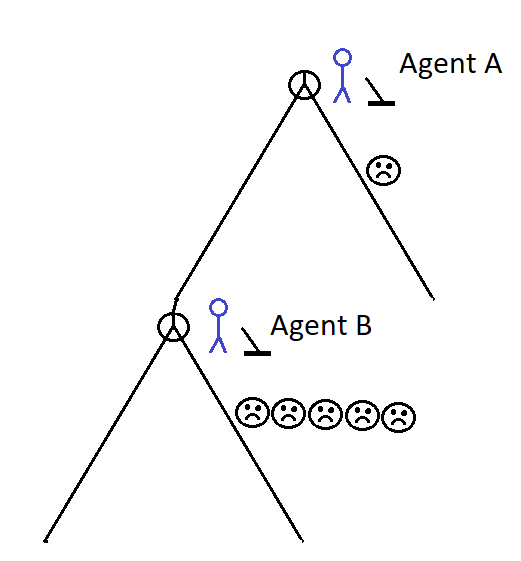
\includegraphics[scale=1]{extended1}
\end{figure}
\end{frame}


\begin{frame}
\frametitle{Example 1: Double trolley problem}
\[
\Pi = \left( \Theta, T, u, \right)
\]
\[
\Theta=(\pi_A, \pi_B)
\]
\[
\pi_A = (V_A, I_A, O_A, \gamma_A)
\]
\[
\pi_B = (V_B, I_B, O_B, \gamma_B)
\]
\[
V_A = V_B = {man, men, tram, leverA, leverB}
\]

\[
O_A = \{pullA, advanceA\}
\]
\[
pullA = (\top, leverA=l \triangleright leverA=r \land leverA=r \triangleright leverA=l)
\]
\[
O_B = \{pullB, advanceB\}
\]
\[
pullB = (\top, leverB=l \triangleright leverB=r \land leverB=r \triangleright leverB=l)
\]

\[
s_0 = (man=alive \land men=alive \land tram = start \land leverA = r, land leverB = r)
\]
\[
\gamma_A=\gamma_B = *
\]
\end{frame}

\begin{frame}
\frametitle{Example 1 analysis}

What constitutes a morally permissible planning task?
\begin{itemize}
\item In single-agent setting: sufficient to show that the action sequence does not lead to or result in the agent performing an action that is morally impermissible.
\item In multi-agent setting: potential for more nuanced evaluation on a \textit{per agent} basis.
\end{itemize}
\begin{definition}
A single-agent plan $\pi$ is morally permissible, according to the deontological principle, iff for all $a_i$, $u(a_i) \geq 0$
\end{definition}
\begin{itemize}
\item By this definition, as in the single-agent case, all possible plans are permissible as no action in this example is intrinsically bad.
\item Things change with our second example.
\end{itemize}
\end{frame}




\begin{frame}
\frametitle{Example 2: Double trolley fat-man problem}


\begin{figure}
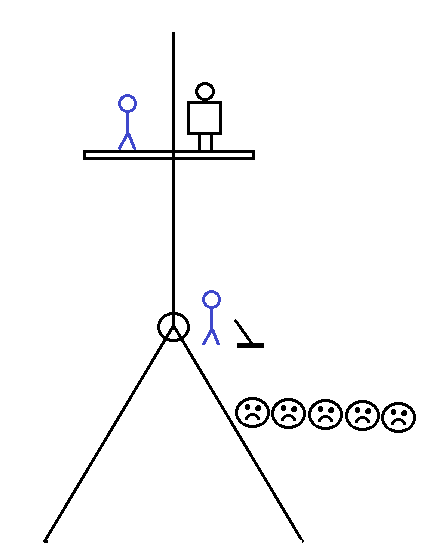
\includegraphics[scale=1]{extended2}
\end{figure}
\end{frame}

\begin{frame}
\frametitle{Example 2: Double trolley fat-man problem}
\[
\Pi = \left( \Theta, T, u, \right)
\]
\[
\Theta=(\pi_A, \pi_B)
\]
\[
\pi_A = (V_A, I_A, O_A, \gamma_A)
\]
\[
\pi_B = (V_B, I_B, O_B, \gamma_B)
\]
\[
V_A = V_B = {man, men, leverB}
\]

\[
O_A = \{pushA, advanceA\}
\]
\[
pushA = (man=onBridge \triangleright man = deadOnTrack)
\]
\[
O_B = \{pullB, advanceB\}
\]
\[
pullB = (\top, leverB=l \triangleright leverB=r \land leverB=r \triangleright leverB=l)
\]

\[
s_0 = (man=alive \land men=alive \land tram = start \land, land leverB = r)
\]
\[
\gamma_A=\gamma_B = *
\]
\end{frame}


%=======================DEONTIC=========================================================


\begin{frame}
\frametitle{Example 2 analysis}
\begin{definition}
A plan $\pi$ is morally permissible, according to the deontological principle, iff for all $a_i$, $u(a_i) \geq 0$
\end{definition}

\begin{itemize}
\item By this definition, any plan that involves the action $push$ is will be morally impermissible.
\item However, from the perspective of Agent B, any action he takes is not impermissable, and no action he takes could have prevented Agent A from performing the $push$ action.
\item Perhaps it is worth distinguishing between overall permissibility of a planning task and permissibility of a planning task wrt. some agent or set of agents within that planning task.
\end{itemize}
\end{frame}

\begin{frame}
\frametitle{Multi-agent Moral Permissibility (Naive Formulation)}
\begin{definition}
A multi-agent plan $\pi$ is morally permissible according to the deontological principle iff, for all agent-action pairs $(X,a_i)$, $u(a_i) \geq 0$.
\end{definition}


\begin{center}
\begin{tabular}{ |c|c| } 
 \hline
 $\pi=$ &  Overall \\ 
 \hline
 $(A,push), (B, pull)$ & $\bot$\\ 
 \hline
 $(A,push), (B, \lnot pull)$ & $\bot$\\ 
 \hline
 $(A,\lnot push), (B, pull)$ & $\top$\\ 
 \hline
 $(A,\lnot push), (B, \lnot pull)$ & $\top$\\ 
 \hline
\end{tabular}
\end{center}

\end{frame}

\begin{frame}
\frametitle{Multi-agent Moral Permissibility (Extended Formulation)}
\begin{definition}
A multi-agent plan $\pi$ is morally permissible wrt. an Agent X, according to the deontological principle iff, for all agent-action pairs $(X,a_i)$, $u(a_i) \geq 0$.
\end{definition}

\begin{definition}
A multi-agent plan $\pi$ is morally permissible, according to the deontological principle iff, for all Agents X, the partial plan for agent X is morally permissible.
\end{definition}


\begin{center}
\begin{tabular}{ |c|c|c|c| } 
 \hline
 $\pi=$ & wrt. A & wrt. B & Overall \\ 
 \hline
 $(A,push), (B, pull)$ & $\bot$ & $\top$ & $\bot$\\ 
 \hline
 $(A,push), (B, \lnot pull)$ & $\bot$ & $\top$ & $\bot$\\ 
 \hline
 $(A,\lnot push), (B, pull)$ & $\top$ & $\top$ & $\top$\\ 
 \hline
 $(A,\lnot push), (B, \lnot pull)$ & $\top$ & $\top$ & $\top$\\ 
 \hline
\end{tabular}
\end{center}

\end{frame}

\begin{frame}
\frametitle{Multi-agent deontic expressiveness}
\begin{theorem}
Multi-agent action plans are order-independent in the deontic case of ethical evaluation.
\end{theorem}
\begin{proof}
Given a deontically valid multi-agent action plan $\pi$, by definition: $\nexists_{a_i \in \pi} u(a_i) \leq 0$.\\
By contradiction:\\
Assume the above holds for $\pi$ but not for $\pi'$, which is a permutation of $\pi$.\\
Then $\exists_{a\in \pi'} u(a_i)<0$.\\
But $\forall_{x_i \in \pi'} x_i \in \pi$ (by definition of permutation).\\
Therefore, $\exists_{a_i \in \pi} u(a_i)<0$.\\
A contradiction.
\end{proof}
\end{frame}


\begin{frame}
\frametitle{Multi-agent deontic expressiveness}
\begin{theorem}
The multi-agent extended case of the deontic principle is equivalent to the multi-agent naive case of the deontic principle.
\end{theorem}
\begin{proof}
For a multi-agent action plan $\pi$:
$f(\pi,X)=\forall_{(a_i,X) \in \pi} u(a_i)\geq 0$. (extended case definition wrt. Agent $X$)\\
$g(\pi) = \forall_{a_i \in \pi} u(a_i)\geq 0$. (naive case definition)\\
We show $g(\pi)=\forall_{X \in L} f(\pi, L)$.\\
By previous proof it is sufficient to show: $\cup_{X \in L} \textrm{subset}(\pi,X) \cup \{\}=\textrm{set}(\pi)$\\
Specifically we show:  $\cup_{X \in L} \textrm{subset}(\pi,X) \cup \{\} \subseteq \textrm{set}(\pi)$ and $ \textrm{set}(\pi) \subseteq \cup_{X \in L} \textrm{subset}(\pi,X) \cup \{\} $.
\end{proof}
\end{frame}

\begin{frame}
\frametitle{Multi-agent deontic expressiveness}
\begin{theorem}
$\cup_{X \in L} \textrm{subset}(\pi,X) \cup \{\} \subseteq \textrm{set}(\pi)$
\end{theorem}
\begin{proof}
Would be invalid iff:
\begin{itemize}
\item There is an agent, operator pair in $\cup_{X \in L} \textrm{subset}(\pi,X) \cup \{\}$ not in $ \textrm{set}(\pi)$.
\end{itemize}
By contradiction:\\
Assume $\exists_{(a_i,X) \in \textrm{subset}(\pi,X)} X \notin \textrm{set}(\pi)$.\\
But $\textrm{subset}(\pi,X)$ is simply a subset of $\pi$.\\
A contradiction.
\end{proof}
\end{frame}

\begin{frame}
\frametitle{Multi-agent deontic expressiveness}
\begin{theorem}
$\textrm{set}(\pi) \subseteq \cup_{X \in L} \textrm{subset}(\pi,X) \cup \{\}$
\end{theorem}
\begin{proof}
Would be invalid iff:
\begin{itemize}
\item There is an agent, operator pair in $ \textrm{set}(\pi)$ not in $\cup_{X \in L} \textrm{subset}(\pi,X) \cup \{\}$.\\
However $\cup_{X \in L} \textrm{subset}(\pi,X) \cup \{\}$ is a true partition of $\pi$ (by definition).



\end{itemize}
\end{proof}
\end{frame}

\begin{frame}
\frametitle{Do-no-harm in multi-agent planning}
\begin{definition}
A single agent plan $\pi$ is morally permissible according to the do-no-harm principle iff, for all $v=d$, if $s_n \models (v=d)$ and $u(v=d)<0$, then for all plans obtained by deleting a subset of the actions in $\pi$, $v=d$ still holds in the final state.
\end{definition}

\begin{itemize}
\item In a multi-agent plan, open to the same considerations as the deontological approach.
\item What is another agent performs an action with a harmful effect, should that invalidate this agent's adherence to that principle?
\end{itemize}


\end{frame}

\begin{frame}
\frametitle{Do-no-harm in multi-agent planning}

\begin{definition}
A multi-agent plan $\pi$ is morally permissible wrt. Agent X, according to the do-no-harm principle, iff, for all $v=d$, if $s_n \models (v=d)$ and $u(v=d)<0$, then for all plans obtained by deleting a subset of the actions performed by X in $\pi$, $v=d$ still holds in the final state.
\end{definition}

\begin{definition}
A multi-agent plan $\pi$ is morally permissible, according to the do-no-harm principle iff, for all $v=d$, if $s_n \models (v=d)$ and $u(v=d)<0$, then for all plans obtained by deleting a subset of the actions in $\pi$, $v=d$ still holds in the final state.
\end{definition}


\begin{center}
\begin{tabular}{ |c|c|c|c| } 
 \hline
 $\pi=$ & wrt. A & wrt. B & Overall \\ 
 \hline
 $(A,push), (B, pull)$& $\bot$ &  $\top$&  $\bot$ \\ 
 \hline
 $(A,push), (B, \lnot pull)$ & $\bot$ & $\bot$ & $\bot$\\ 
 \hline
 $(A,\lnot push), (B, pull)$ & $\top$ & $\top$ & $\top$\\ 
 \hline
 $(A,\lnot push), (B, \lnot pull)$ & $\top$ & $\bot$ & $\bot$\\ 
 \hline
\end{tabular}
\end{center}

\end{frame}

\begin{frame}
\frametitle{Utalitarianism in multi-agent planning}

\begin{itemize}
\item Significantly harder.
\item If other agents actions are deterministic, then a reduction from the multi-agent to the single agent case can be done in polynomial time.
\item If other agents are random, then average or worst case estimates may suffice.
\item If however, the other agent has actions dependent on the current agent, an intuitive way of distinguishing individual agent contributions to overall moral utility of the final state becomes difficult.
\item Evaluation of ethical contributions of subplans (as in do-no-harm and deontic cases) would only provide a heurisic-like estimate.
\item How would non-determinism be handled in the single-agent case?
\end{itemize}



\end{frame}
















\end{document}

